\phantomsection
\part{証明}

\begin{abstract}
この章では，前章で整理した論理を踏まえて，数学の議論の中心である「証明」を扱う．まず証明とはなにかを確認し，帰納法・背理法・直接証明や反例による反証といったさまざまな証明法を具体例とともに見ていく．そのうえで，数学的主張の骨格をなす「存在」と「一意性」について，「数学では何を証明しなければならないのか」という観点から具体例をもとに整理しよう．
\end{abstract}

\phantomsection
\section{証明とは}
数学において，主張が正しいことを示すプロセスを\emph{証明}\index{しょうめい@証明}（\emph{proof}）という．

\begin{remark}[定義は「証明すべきこと」ではない]
  先の例で，命題・定理・補題・系は証明されるべきものであるが，定義は一般に「証明すべきこと」でないことに注意したい．
  ただし，たとえば「\exref{「絶対値」の定義}において$\abs{x} \coloneqq \max \{ x, -x \}$を仮定して$\abs{x} = \sqrt{x^2}$を導く」など，異なる定義の同値性を示す場面では，定義が「証明すべきもの」となる．このことから，どの定義を採用しているか明確にすることが重要であることがわかる．
\end{remark}

以下で，証明の例をいくつか見てみよう：


\begin{example}{証明①（余りの計算）}{証明①（余りの計算）}
  「任意の奇数$n$について，$n^2$を$4$で割った余りは$1$である」という命題を証明しよう：

  奇数$n$は，ある整数$k$を用いて$n = 2k + 1$と表すことができる．このとき，
\[
  n^2 = (2k + 1)^2 = 4k^2 + 4k + 1 = 4(k^2 + k) + 1
\]
である．したがって，$n^2$を$4$で割った余りは$1$である．これが証明すべきことであった．\qed
\end{example}

このように証明することで，「任意の奇数$n$について，$n^2$を$4$で割った余りは$1$である」という命題が真であることが示され，したがってこの命題の主張は「疑いようのない真実」であることがわかる．

証明はひとつの命題にいくつか存在する場合がほとんどであり，たとえば，\exref{三平方の定理}の証明は100通り以上も存在することが知られている．
数学の学習を進めるにあたって，さまざまな証明を見てみることは，論理的な思考力を養ううえで非常に有益である．

\phantomsection
\begin{example}[
    sidebyside,
    lefthand width=8.5cm,
    righthand width=5cm,
    sidebyside gap=4mm,
  ]{証明（三平方の定理）}{証明（三平方の定理）}
  辺の長さが$a$と$b$の直角三角形を$4$つ用意し，
  これらを組み合わせて，辺の長さが$a + b$の正方形を作る．
  この正方形は，中央の辺の長さが$c$の正方形と$4$つの三角形からなる．

  したがって，面積を2通りに計算すると
  \[
    (a + b)^2
    = c^2 + 4\left(\frac{1}{2}ab\right)
    = c^2 + 2ab
  \]
  である．これを展開して
  \[
    a^2 + 2ab + b^2 = c^2 + 2ab,
    \quad \therefore\quad a^2 + b^2 = c^2
  \]
  を得る．
  これが証明すべきことであった．\qed

  \tcblower

  \centering
  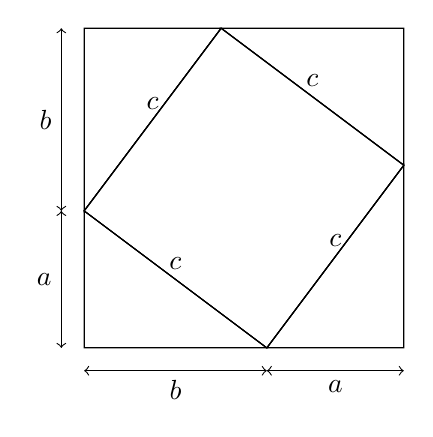
\begin{tikzpicture}[scale=0.58]
    \def\a{3}
    \def\b{4}

    % 大きな正方形
    \draw (0,0) rectangle (\a+\b,\a+\b);

    % 4つの直角三角形
    \draw (0,0) -- (\b,0) -- (0,\a) -- cycle;
    \draw (0,\a) -- node[midway,above] {$c$} (\b,0);

    \draw (\b,0) -- (\a+\b,0) -- (\a+\b,\b) -- cycle;
    \draw (\a+\b,\b) -- node[midway,above] {$c$} (\b,0);

    \draw (\a+\b,\b) -- (\a+\b,\a+\b) -- (\a,\a+\b) -- cycle;
    \draw (\a,\a+\b) -- node[midway,above] {$c$} (\a+\b,\b);

    \draw (\a,\a+\b) -- (0,\a+\b) -- (0,\a) -- cycle;
    \draw (0,\a) -- node[midway,above] {$c$} (\a,\a+\b);

    % 中央の正方形
    \draw (\b,0) -- (\a+\b,\b) -- (\a,\a+\b) -- (0,\a) -- cycle;

    % 寸法
    \draw[<->] (-0.5,0) -- (-0.5,\a) node[midway,left] {$a$};
    \draw[<->] (-0.5,\a) -- (-0.5,\a+\b) node[midway,left] {$b$};
    \draw[<->] (0,-0.5) -- (\b,-0.5) node[midway,below] {$b$};
    \draw[<->] (\b,-0.5) -- (\a+\b,-0.5) node[midway,below] {$a$};
  \end{tikzpicture}
\end{example}


\begin{mycolumn}
  証明を記述する際には，文末に$\square$や$\blacksquare$をかくことが一般的である．そのほかに``Q.E.D.''\footnote{``quod erat demonstrandum''の略で，ラテン語で「証明されるべきであったこと」という意味である．}などの表現も用いられる．
\end{mycolumn}

\phantomsection
\section{さまざまな証明法}

命題が真であることを示す方法にも，偽であることを示す方法にも，さまざまなものがある．代表的なものを挙げてみよう．

\begin{description}[descnext]
  \item[帰納法\index{きのうほう@帰納法}]
        たとえば数学的帰納法は，数学的な主張が自然数全体に対して成り立つことを示すための証明法である．
  \item[背理法\index{はいりほう@背理法}]
        「$P$が成り立たないと仮定すると矛盾が生じる」という論理的な構造を用いて証明を行う方法である．
  \item[直接証明\index{ちょくせつしょうめい@直接証明}]
        「$P$が成り立つことを示す」という形式で証明を行う方法である．
  \item[反例による反証\index{はんれい@反例}]
        全称命題「すべての$x$について$P(x)$が成り立つ」が\textbf{偽}であることを示すには，$P(x)$が成り立たない$x$，すなわち\emph{反例}をひとつ挙げれば十分である．
\end{description}

以下では，まず「$n \geqq 2$ を満たす任意の自然数について，$2^n > n$である」という命題を3通りのやり方で証明してみよう．

\phantomsection
\begin{example}{帰納法}{帰納法}
  \begin{enumerate}[(I)]
    \item $n=2$のとき，
          \[
            2^2 = 4 > 2
          \]

          となり，与えられた不等式は成立する．
    \item 自然数$k$を$k \geqq 2$を満たすように任意にとる．$2^k > k$ が成り立つと仮定する．このとき，
          \[
            2^{k+1} = 2 \cdot 2^k > 2k
          \]
          である．
          ここで，$k \geqq 2$であるから，$2k - (k + 1) = k - 1 \geqq 1$であるがゆえに，$2k > k + 1$である．

          したがって，

          \[
            2^{k+1} > 2k > k + 1
          \]
          である．
          ゆえに，$n=k+1$のときも$2^{k+1} > k + 1$である．
  \end{enumerate}

  以上の考察と数学的帰納法により，$2^n > n$ は $n \geqq 2$を満たすすべての自然数について成り立つ．これが証明すべきことであった．\qed
\end{example}

\phantomsection
\begin{example}{背理法}{背理法}
  $n \geqq 2$を満たす自然数で $2^n \leqq n$ となるものが存在すると仮定する．
  $2^n$ の正の約数の個数は，指数に $1$ を加えたものなので，$2^n$の正の約数の個数は $n + 1$ 個以上である．
  しかし，仮定より $2^n \leqq n$ なので，$2^n$ は $n$ 以下の数である．

  これは，$n$ 以下の数が $n + 1$ 個以上の正の約数を持つことを意味するが，これは矛盾である．

  したがって，先の仮定が誤りであるため，背理法によって$2^n > n$ が成り立つ．これが証明すべきことであった．\qed
\end{example}

\phantomsection
\begin{example}{直接証明}{直接証明}
  \[
    2^n = n \int_{1}^{2} x^{n-1} \, dx + 1
  \]
  となることはよい．さて，$x \in [1, 2]$ かつ $n \geqq 2$ なので，
  \[
    x^{n-1} \geqq x^{1} \geqq 1
  \]
  が成り立つ．したがって，
  \begin{align*}
    2^n & = n \int_{1}^{2} x^{n-1} \, dx + 1 \\
        & \geqq  n \int_{1}^{2} \, dx +1     \\
        & = n+1
  \end{align*}
  である．
  これと$n+1 >n$であることを併せると，$n \geqq 2$のとき$2^n > n$である．これが証明すべきことであった．\qed
\end{example}

最後に，反例による反証の例を見てみよう．全称命題は「すべての場合において成り立つ」ことを主張しているため，ひとつでも例外があれば命題全体が偽となる．したがって，命題が偽であることの証明としては，反例をひとつ示すだけで十分なのである．

\phantomsection
\begin{example}{反例による反証}{反例による反証}
  次の命題を考える：
  \[
    \forall n \in \mathbb{N}\, : \, \frac{n^3}{24} + 84 \geqq n^2
  \]
  この命題が成り立たないことを示すためには，ある$n$について不等式が成立しないことを示せばよい．実際に，$n = 15$のとき，
  \[
    \frac{15^3}{24} + 84 = \frac{3375}{24} + 84 = 140.625 + 84 = 224.625
  \]
  である．
  一方，
  \[
    15^2 = 225
  \]
  である．
  したがって，
  \[
    \frac{15^3}{24} + 84 = 224.625 < 225 = 15^2
  \]
  が成り立つ．
  このように，$n = 15$において不等式が成り立たないため，元の命題は偽であることがわかる．
\end{example}

また，全称命題が偽であることを証明する際には，「反例をどう見つけたか」ということは明記しない場合が多い．
たとえば\exref{反例による反証}の場合に$n=15$を見つけるには，微分法を用いて議論したりさまざまな方法があるが，そのような「反例を見つけるまでの過程」を説明する必要はなく，「$n=15$の場合に命題が成り立たないこと」のみを証明として書けばよい．

\phantomsection
\section{数学における存在と一意性}

ここまでで，証明とはなにか，そしてどのような証明法があるかを確認した．
本節では，数学的な主張そのものの論理構造に一歩踏み込み，「存在する」という主張と「ただひとつである」という主張について考える．
これらは単なる言い回しではなく，「数学では何を証明しなければならないのか」を決める骨格である．

\phantomsection
\subsection{存在}

数学の証明において，「存在\index{そんざい@存在}」は重要な概念である．といっても，あまりこのことを意識したことのない読者の方もいると思うので，この場を借りて具体例をもとに説明を試みることとする．

まず，以下に記す「最大値・最小値の定理」を考える：
\begin{quotation}
  $[a,b]$で連続な関数$f$に対して，$f$は$[a,b]$上で最大値と最小値を持つ．
\end{quotation}

「最大値・最小値が存在するなんて当たり前だ」と思われる読者もいるかもしれない．しかし，本当にそれは自明なのか．
実際には，関数の連続性や区間の閉有界性といった条件が揃って初めて，最大値や最小値の「存在」を保証できる．この定理を証明するにあたっては，厳密な数学的議論が必要となる．

「存在」の重要性がわかる例として，「極限値の存在」に関する命題を以下で考えてみよう：

\begin{prop}{}{}
  以下のような漸化式で定められた数列$(x_n)_{n \in \mathbb{N}}$を考える：
  \[
    \begin{cases}
      x_1 =0 , \\
      x_{n+1}= \sqrt{x_n+2}
    \end{cases}
  \]
  このとき，$(x_n)_{n \in \mathbb{N}}$は収束し，極限値は次のようになる：
  \[
    \lim_{n \to \infty} x_n =2
  \]
  が成り立つ．
\end{prop}

\begin{tleftbar}
  \begin{proof}
    いくつかの補題を確認しつつ示す．
    \begin{lemma}{}{}
      任意の$n \in \mathbb{N}$に対して，以下の不等式が成り立つ：
      \[
        x_n \leqq x_{n+1} < 2
      \]
    \end{lemma}
      \begin{proof}
        数学的帰納法により，$x_n \leqq x_{n+1} < 2$を示す．
        \begin{enumerate}[(I)]
          \item \mbox{} \\ \label{proof:存在1}
                $n=1$のとき，$ x_1 =0$，$x_2= \sqrt{0+2}=\sqrt{2}$なので，$ 0 \leqq \sqrt{2} < 2$により，
                $x_1 \leqq x_2 < 2$である．
          \item \mbox{} \\ \label{proof:存在2}
                $k \in \mathbb{N}$を任意にとり，$x_k \leqq x_{k+1} < 2$であると仮定する．

                このとき，$x_{k+1} < 2$により$ x_{k+1}+2 < 4$なので，以下の式が成り立つ：
                \[
                  x_{k+2}=\sqrt{x_{k+1} + 2} < 2
                \]

                また，$x_k \leqq x_{k+1}$により，$x_k +2  \leqq x_{k+1}+2$であるから，
                \[
                  x_{k+1}= \sqrt{x_k +2} \leqq \sqrt{x_{k+1}+2}=x_{k+2}
                \]
                が成り立つ．
                よって，$n=k+1$の場合にも成り立つ．
        \end{enumerate}
        以上\ref{proof:存在1}，\ref{proof:存在2}により，任意の$n \in \mathbb{N}$について，以下の不等式が成り立つ：
        \[
          x_n \leqq x_{n+1} < 2.
        \]
      \end{proof}
    \begin{lemma}{}{}
      $(x_n)_{n \in \mathbb{N}}$は$ 0<  x \leqq 2$なる極限$x$に収束する．
    \end{lemma}
      \begin{proof}
        先の補題により，任意の$n \in \mathbb{N}$について，$ x_n \leqq x_{n+1} <2$なので，
        数列$(x_n)_{n \in \mathbb{N}}$は単調に増加し，上に有界である．

        よって
        \[
          x \coloneqq \sup \{ x_n \mid n \in \mathbb{N} \}
        \]
        が存在し，$x \leqq  2$である．

        $ x>0$は明らかである．これが証明すべきことであった．
      \end{proof}

    ここまでで，$(x_n)_{n \in \mathbb{N}}$の極限値の存在が確認されたので，先の漸化式について，
    \[
      x=\sqrt{x+2}
    \]
    とする．これを解くと$ x= -1,2$であるが，$x>0$により$x=2$である．

    以上の考察により，数列$(x_n)_{n \in \mathbb{N}}$は収束し，
    \[
      \lim_{n \to \infty} x_n =2
    \]
    が成り立つ．これが証明すべきことであった．
  \end{proof}
\end{tleftbar}

ここまで考察して，ようやく数列$(x_n)_{n \in \mathbb{N}}$が収束することを確認できた．
この例では「極限値の存在」を確認する意味がわからない読者もいるかもしれないので，もうひとつ例を挙げよう．


以下のような漸化式で定められた数列$(y_n)_{n \in \mathbb{N}}$を考える：
\[
  \begin{cases}
    y_1 =1 , \\
    y_{n+1}= 2y_n +2
  \end{cases}
\]
この数列の極限値が存在すると仮定して，それを$y$とおこう．
\begin{tleftbar}
  与えられた漸化式により，
  \begin{align*}
     & y = 2y +2,           \\
     & \therefore ~ y = -2.
  \end{align*}
  しかし，
  \[
    \lim_{n \to \infty} y_n = \infty
  \]
  なので，$y=-2$は誤りである．
\end{tleftbar}

このように，数列の極限が存在することを確認しないと，誤った結論に到達することがある．この例からわかるように，存在を確認することは重要なことなのである．


\phantomsection
\subsection{一意性}

\begin{wrapfigure}[10]{r}{0.425\textwidth}
  %\centering
  \begin{tikzpicture}[scale=0.78]
    \begin{axis}[
        axis lines=middle,
        xmin=-1.2, xmax=1.2,
        ymin=-1.5, ymax=1.5,
        xtick=\empty, ytick=\empty, % 目盛を消す
        xlabel={}, ylabel={},       % ラベルを消す
        samples=200,
        domain=-1.2:1.2,
        width=10cm,
        height=8cm,
      ]
      % 関数 f(x) = x^3 のグラフ
      \addplot [dblue, thick] {x^3};

      % 点 (-1, -1) と (1, 1) を結ぶ割線
      \addplot [dred, thick] coordinates {(-1, -1) (1, 1)};

      % 平均値の定理を満たす点 x = -1/√3 の接線
      \def\xone{-1/sqrt(3)}
      \def\yone{(\xone)^3}
      \addplot [dgreen, dashed] {1*(x - \xone) + \yone};

      % 平均値の定理を満たす点 x = 1/√3 の接線
      \def\xtwo{1/sqrt(3)}
      \def\ytwo{(\xtwo)^3}
      \addplot [dgreen, dashed] {1*(x - \xtwo) + \ytwo};

      % 重要な点をマーク
      \addplot [only marks, mark=*, mark options={fill=black}] coordinates {(\xone, \yone) (\xtwo, \ytwo)};
      \addplot [only marks, mark=*, mark options={fill=dred}] coordinates {(-1, -1) (1, 1)}; % 赤い丸に変更
    \end{axis}
  \end{tikzpicture}
\end{wrapfigure}

読者の中には線型代数の講義で「逆行列の一意性」などに触れた方もいると思われる．線型代数以外の分野でも，数学の学習を進める際に，「一意性\index{いちいせい@一意性}」が重要である場面は多い．なぜ「一意性」が重要であるのか，ひとつ例を挙げて考えてみることにしよう．

微分積分の講義で習う定理に「平均値の定理」というものがある．
その主張は
\begin{quotation}
  $[a,b]$で連続，$(a,b)$で微分可能な関数$f$に対して，
  \[
    \frac{f(b)-f(a)}{b-a}=f'(c)
  \]
  を満たす$ c \in (a,b)$が存在する．
\end{quotation}

というものである．証明はのちに述べるとして，この定理の主張を少し変更してみよう：

\begin{quotation}
  $[a,b]$で連続，$(a,b)$で微分可能な関数$f$に対して，
  \[
    \frac{f(b)-f(a)}{b-a}=f'(c)
  \]
  を満たす$ c \in (a,b)$がただひとつ存在する．
\end{quotation}


ここで「$c \in (a,b)$が存在する」という主張を「$c \in (a,b)$がただひとつ存在する」というより強い主張に変更した．この主張は偽である．このことが問題になる状況を挙げよう．
$f(x)=x^3$という関数を考える．この関数は$[-1,1]$で連続，$(-1,1)$で微分可能である．
このとき，図のように，条件を満たす$c \in (-1,1)$は複数存在するので，「ただひとつ存在する」という主張は偽である．
さらに言えば，2本より多くこのような接線を引ける場合もある\footnote{各自で確認してみてほしい．}．

このことから，安易に「ただひとつ存在する」などと強い主張をすることは避けるべきであることがわかる．このことは平均値の定理に限らず，中間値の定理なども同様である．

\phantomsection
\subsection{存在と一意性の違い}

ここまでの考察からわかるように，「存在する」という主張と「ただひとつである」という主張は，別々に考える必要がある．
とくに，一意性を示すことは，それ自体では存在を保証しない．
典型的な例を整理すると，次のようになる．

\begin{center}
  \begin{tabular}{|c|p{9.5cm}|}
    \hline
    \textbf{状況} & \textbf{例} \\ \hline

    存在し，一意である
    &
    正則行列\footnote{逆行列を持つ正方行列のことを正則行列という．}の逆行列，
    方程式$x^3 = 8$の実数解など．
    \\ \hline

    存在するが，一意ではない
    &
    方程式$x^2 = 4$の実数解など．
    また，平均値の定理によって存在が保証される$c$も，一般には一意とは限らない．
    \\ \hline

    存在しない
    &
    方程式$x^2 = -1$の実数解など．
    \\ \hline

    一意性だけが示されている
    &
    存在するかどうかとは別に，
    「もし存在するなら，それはただひとつである」とだけ示されている場合である．
    \prref{逆行列の一意性}がこの形の主張である．
    \\ \hline
  \end{tabular}
\end{center}

したがって，ある対象が「ただひとつ存在する」ことを示すには，
\textbf{存在性}と\textbf{一意性}の両方を示さなければならない．

\begin{remark}[「存在」と「一意性」は別の課題]
  とくに，「一意性だけが示されている」場合に注意しよう．
  \prref{逆行列の一意性}をあらためて見返すと，
  「存在するとすれば」とあるように，この命題は逆行列の存在を一切主張していない．
  実際，逆行列を持たない正方行列は存在する\footnote{たとえば零行列．}．
  このように，一意性の証明は存在の証明と切り離して，ときには存在の証明よりも先に行うことができる．
  「存在」と「一意性」は，証明においても別々に扱われるべきふたつの課題なのである．
\end{remark}

% NOTE: この部は執筆中（今後，節を追記する可能性あり）
